\documentclass{article} % \documentclass{} is the first command in any LaTeX code.  It is used to define what kind of document you are creating such as an article or a book, and begins the document preamble

\usepackage{amsmath} % \usepackage is a command that allows you to add functionality to your LaTeX code
\usepackage{graphicx} % allows for images to be added to the latex document

\usepackage{hyperref} % allows for hyperlinks to be added to the document
\hypersetup{
    colorlinks,
    citecolor=black,
    filecolor=black,
    linkcolor=black,
    urlcolor=black
}

\usepackage[
backend=biber,
style=alphabetic,
sorting=ynt
]{biblatex} %Imports biblatex package
\addbibresource{references.bib} %Import the bibliography file

\graphicspath{{../pdf/}{./research_images}}

\title{Research} % Sets article title
\author{Sean Groenenboom \and Seger Sars \and Siem Vermeulen \and Angel Villanueva \and Ronan Vlak} % Sets authors name
\date{\today} % Sets date for date compiled
\newpage
\begin{document}

\maketitle % creates title using information in preamble (title, author, date)
\newpage

\tableofcontents % creates a table of contents
\newpage

\section{Seger}

\subsection{gamespeed}
How do game engines handle game speed?
\subsection{2d rendering}
How do game engines render 2d graphics?
\subsection{sprites}
How do game engines handle sprites?
\newpage
\section{Game speed}
Movement is a very important part of any game, but how is movement calculated accurately across different computers?
Different computers have different internals and thus run games with differing performance.
One computer might be able to run the games at 60FPS, but another can only run the game at 30FPS.
How can you make sure that both users have the exact same experience despite the difference in render speed.
A difference in render speed is shown in figure \autoref{fig:TimeBetweenFramesDisplayed} below.
\begin{figure}[h!]
	\centering
	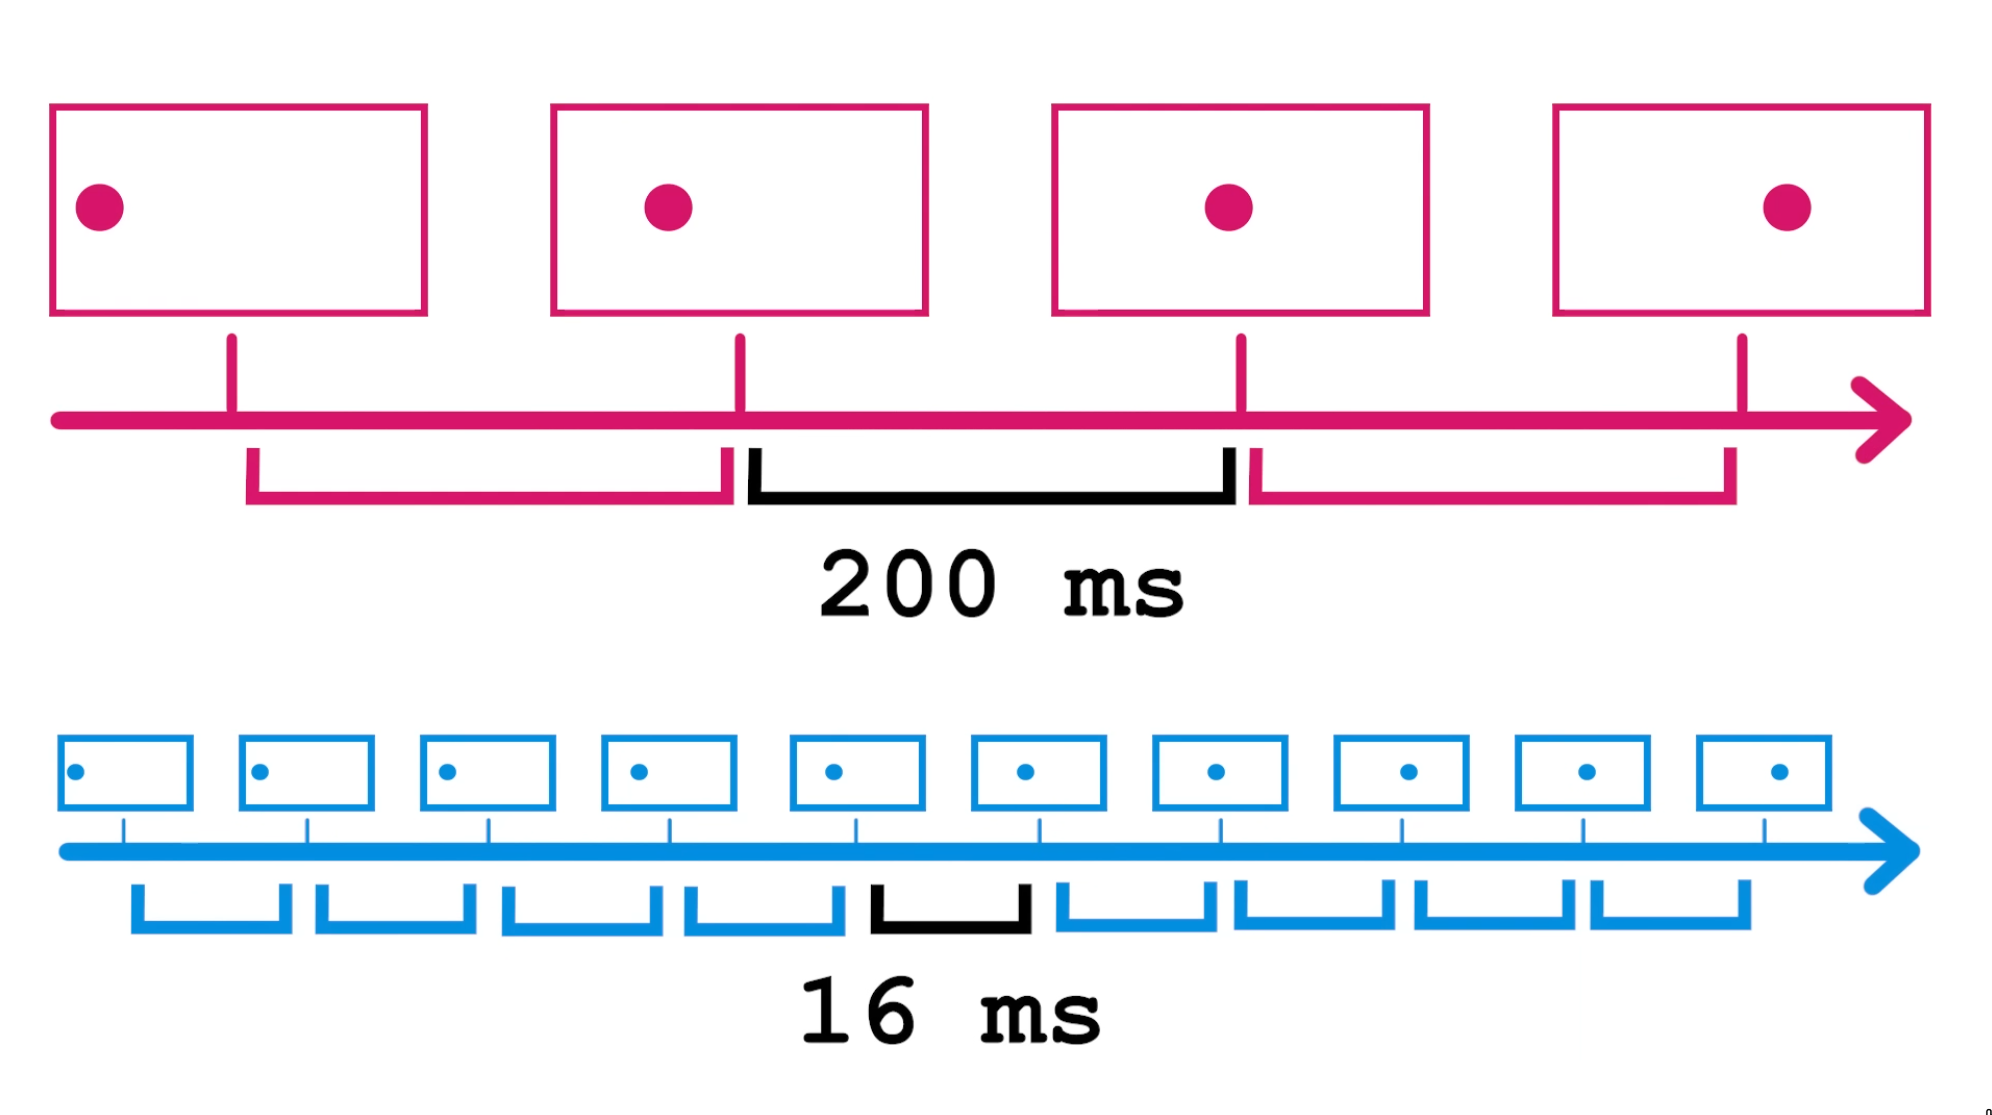
\includegraphics[width=0.8\textwidth]{time_between_frames.png}
	\caption{Time between frames displayed}
	\label{fig:TimeBetweenFramesDisplayed}
\end{figure}

\subsection{Potential problems}
A standard game loop runs one time each frame, before the frame is rendered.
The game loop is responsible for handling all the movement in the game, like moving the player.
If the game runs at 60FPS the game loop will be run 60 times each second.
\newline\newline
The following formula could be used to move the player each game loop iteration:
\newline
playerPosition.x = playerPosition.x + 10
\newline\newline
If this formula would be used to move the player, when running at 60PFS, the player would move 600 units of length each second.
But if the game was running at 30FPS, the player would only move 300 units each second.
So the player with 60FPS is considerably faster than the one with 30FPS.
This is of course, not ideal, as a game developer you want everyone to move at the same speed despite the computer it is run on.
The difference in elapsed distance is also shown in the \autoref{fig:DifferenceInElapsedDistance} below.
\begin{figure}[h!]
	\centering
	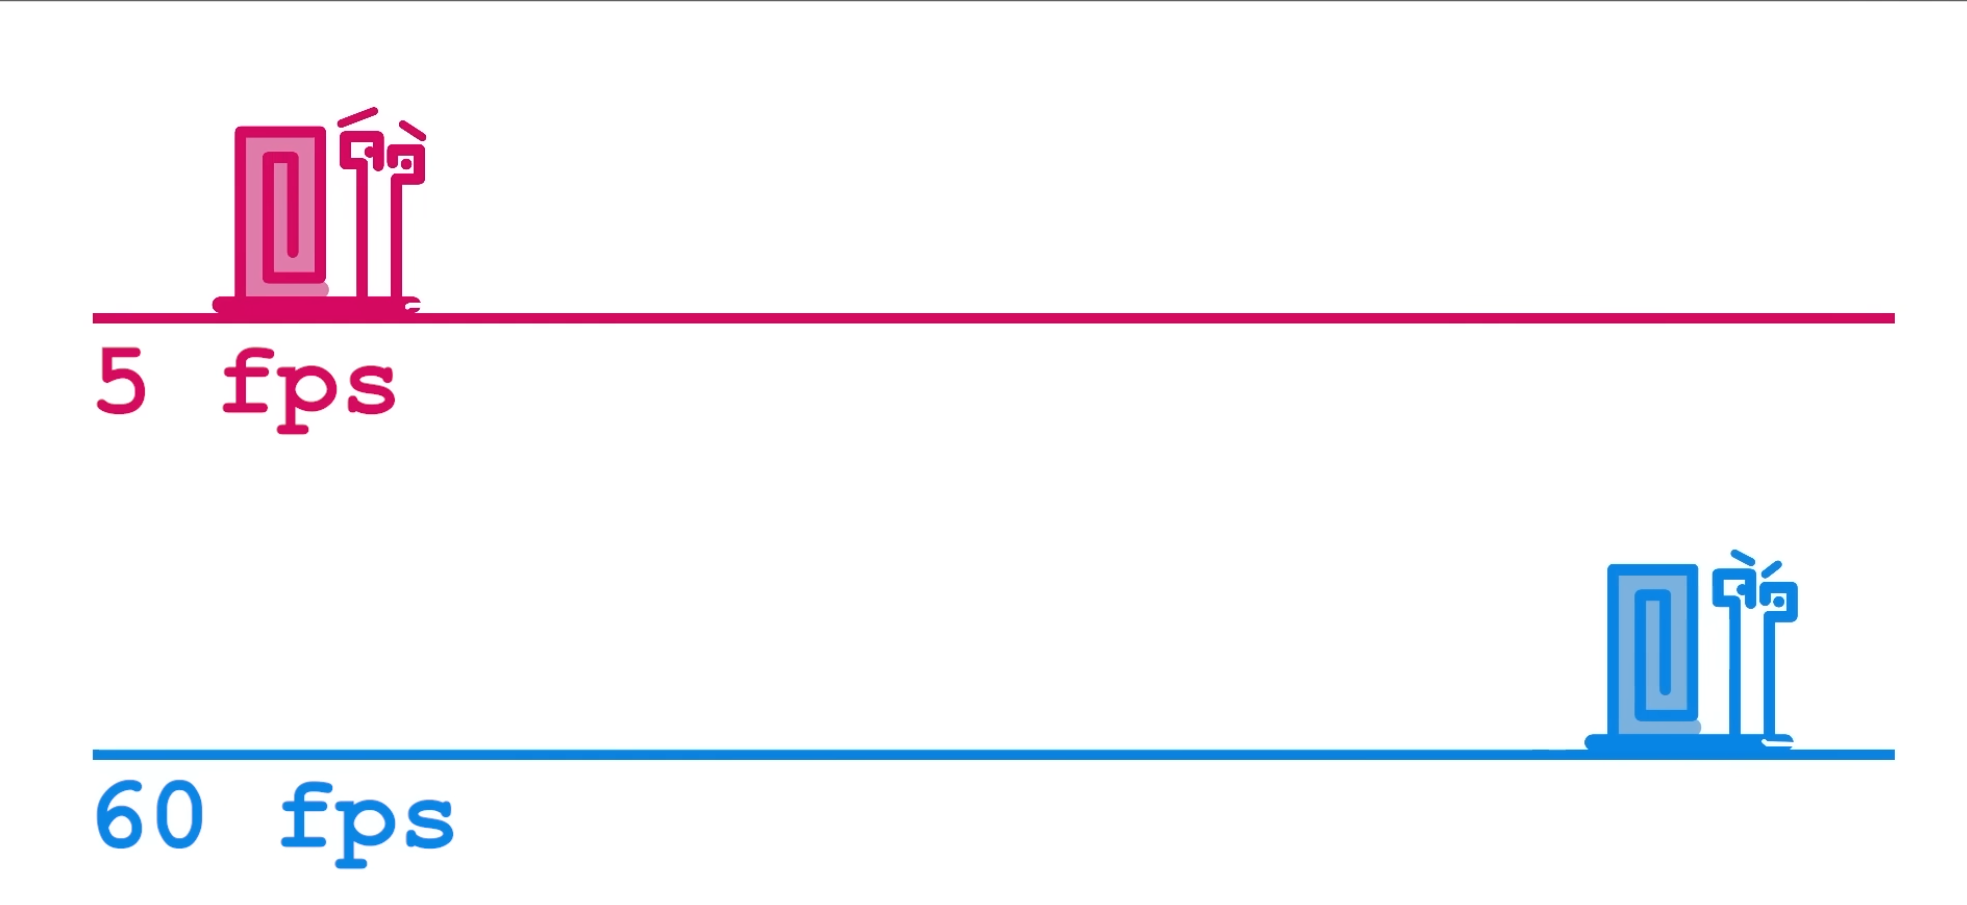
\includegraphics[width=0.8\textwidth]{difference_in_distance.png}
	\caption{Difference in elapsed distance}
	\label{fig:DifferenceInElapsedDistance}
\end{figure}

\subsection{Possible solutions}
There are two common solutions that help alleviate this problem, adjusting the movement speed relative to the FPS or making sure to handle movement in a fixed update loop that is guaranteed to run at a certain amount of cycles each second.

\subsubsection{Fixed update}
A solution to the differing movement speeds between computers, is to create a lightweight time based interrupt, often referred to as FixedUpdate, to handle all movement.
It is important that the FixedUpdate function is very small, otherwise the FixedUpdate could be too slow to be called at a constant rate each frame, defeating the purpose of the FixedUpdate.
In the \autoref{fig:FixedUpdateView} below it is shown how times between different rendered frames can vary, while the FixedUpdate is called at a constant rate, where the small black bar represents the duration of the FixedUpdate function.
\begin{figure}[h!]
	\centering
	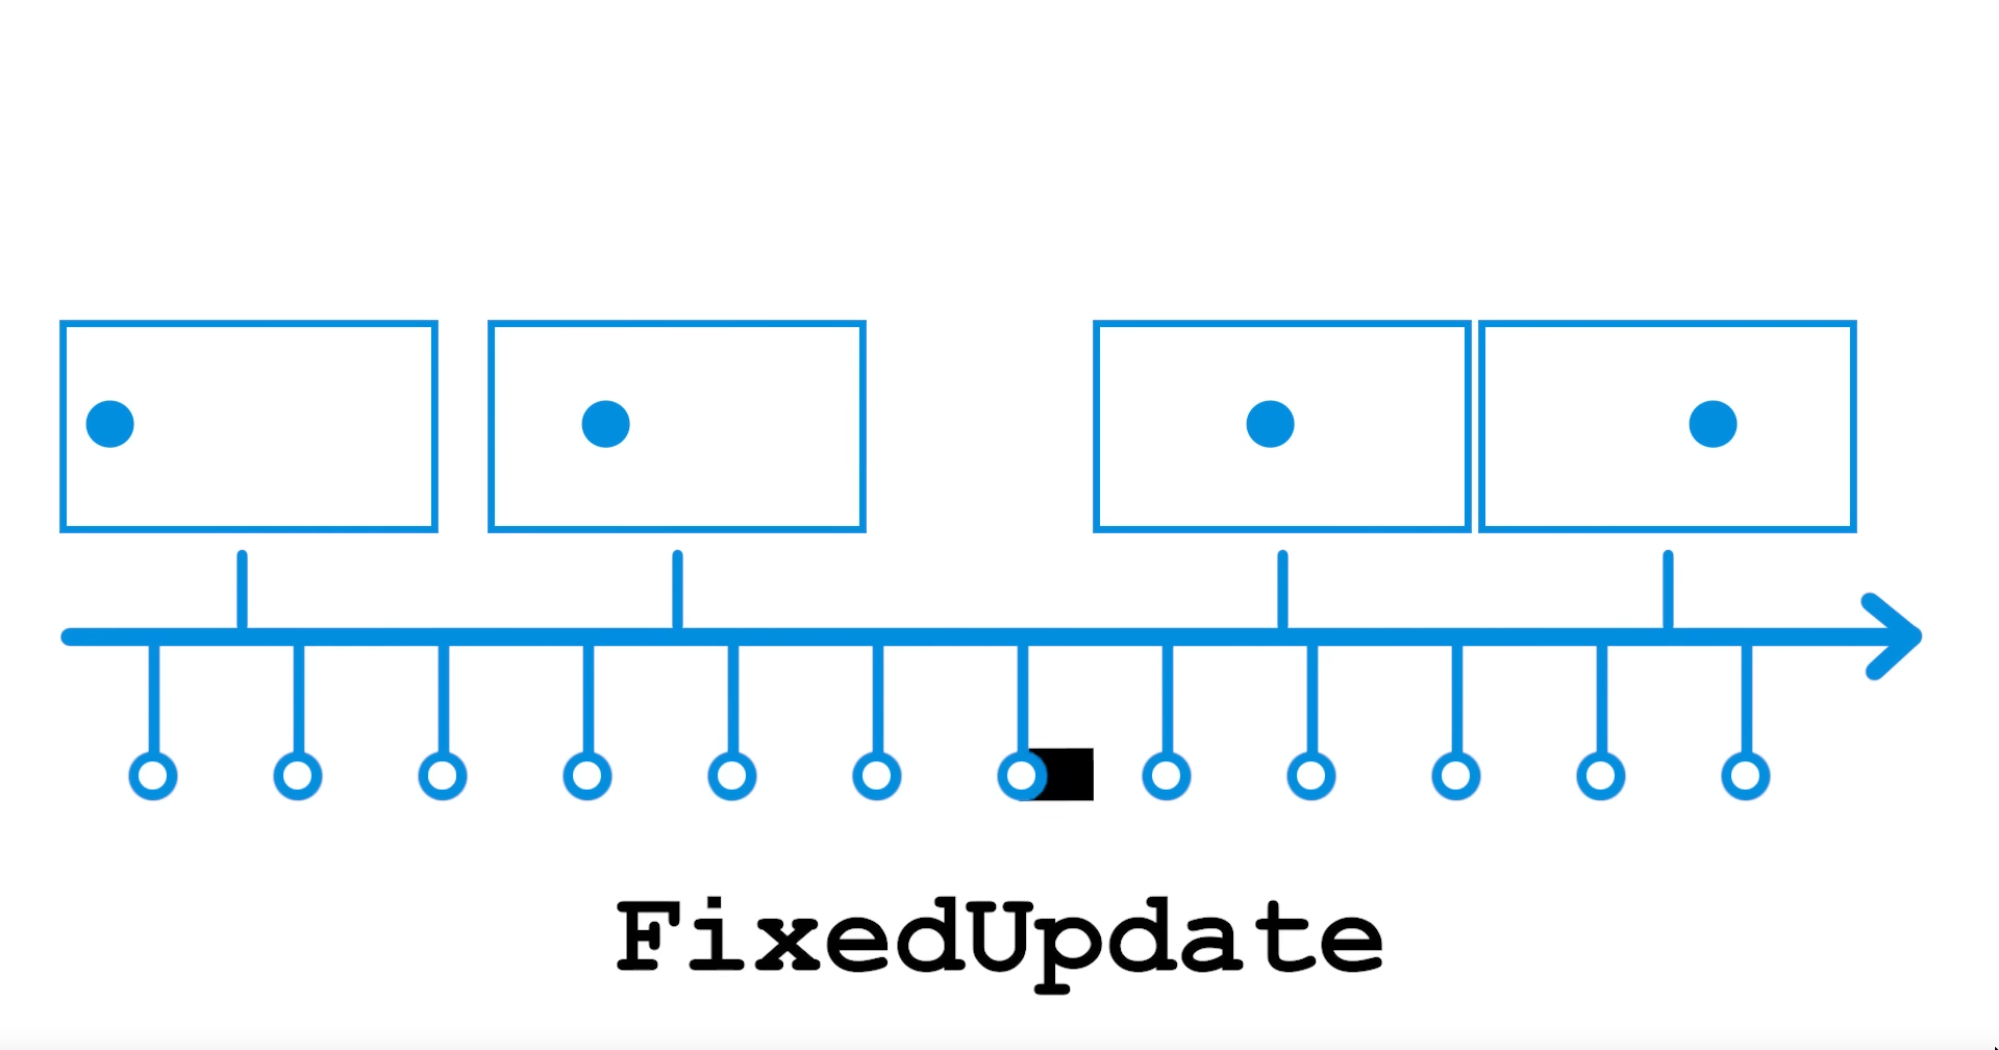
\includegraphics[width=0.6\textwidth]{fixed_update_explanation.png}
	\caption{Fixed update view}
	\label{fig:FixedUpdateView}
\end{figure}
\newline
If you were to use the same formula to calculate the player movement as before, it would now show constant movement between computers.

\subsubsection{Delta time}
Another solution to the differing speeds between computers, is to make the added distance when moving the player relative to the last time distance was added to the player.
Keeping track of every time movement is added to an object is not very efficient so this is solved in a slightly different manner.
So this means the formula would look like this:
\newline
playerPosition.x = playerPosition.x + (10 * deltaTime)
\newline
This uses the deltaTime variable to make the movement relative to the last time the movement was calculated.
\newline\newline
The deltaTime variable is calculated by the game engine and is globally accessible.
The game engine measures the time between the previous frame and the frame before, then assigns that value to the deltaTime variable.
This process is shown in the image below where the black square is the place deltaTime is used and the 0.14 is the time it took for the previous frame to render.
\begin{figure}[h!]
	\centering
	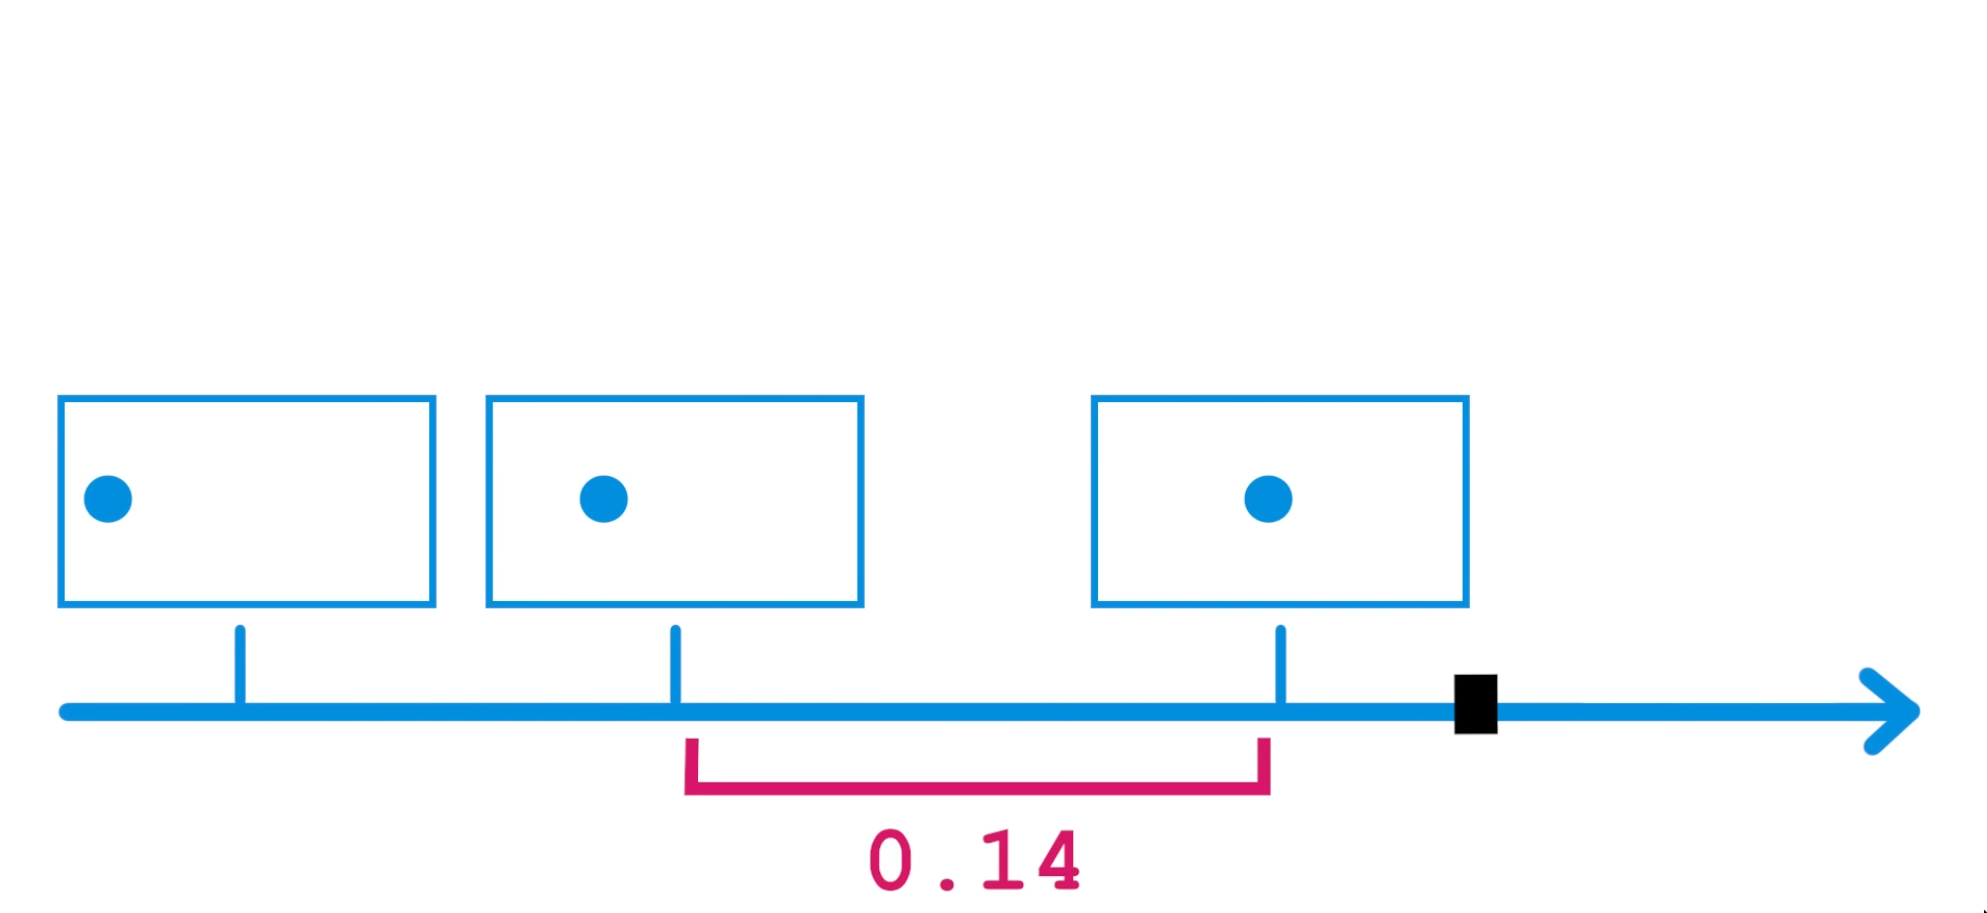
\includegraphics[width=0.6\textwidth]{used_deltatime_when_using_variable.png}
	\caption{deltaTime value when using variable}
\end{figure}
\newline
Because deltaTime is used while rendering a frame, it is not possible to know how long it takes to render the rest of the frame.
This is why the value for the previous frame is used, although this means the deltaTime value lags behind by one frame, the delay is not noticable in most situations.

\newpage
\section{sean}
\subsection{Multiplayer}
Whhich are frequently used multiplayer structures?
\subsection{input}
How do game engines handle input?
controller
\subsection{ai}
What kind of ai do game engines usually have?
pathfinding?
\newpage

\section{multiplayer}
Multiplayer is an important aspect of gaming. It is not necessary for a game to work, but it can greatly enhance the experience.
\subsection{models}
There are multiple multipayer models each with their own advantages and disadvantages.

\subsubsection{Client-Server Model}
The \textit{client-server} model is one of the most widely used architectures for multiplayer games. In this model, a server hosts the game world, and clients (players) connect to it. The server is considered authoritative, managing the game state and ensuring consistency across all clients.

\textbf{Advantages}
\begin{itemize}
	\item Ensures a consistent and authoritative game state.
	\item Reduces the risk of cheating, as the server controls the game logic.
	\item Scalable for large games (e.g., MMOs).
\end{itemize}

\textbf{Challenges}
\begin{itemize}
	\item Requires a reliable and performant server, which adds complexity and cost.
	\item Introduces latency between clients and the server, which can affect gameplay responsiveness.
\end{itemize}

\subsubsection{Peer-to-Peer (P2P) Model}
In the \textit{peer-to-peer} model, all players (peers) are directly connected to each other, and the game state is shared among them. Each peer has equal authority over the game, which can make synchronization and consistency more difficult to maintain.

\textbf{Advantages}
\begin{itemize}
	\item Simple to implement for small-scale games with a limited number of players.
	\item No need for a dedicated server, reducing costs.
\end{itemize}

\textbf{Challenges}
\begin{itemize}
	\item Difficult to ensure game state consistency across peers.
	\item Susceptible to cheating, as each peer has authority.
	\item Latency and synchronization issues are harder to manage.
\end{itemize}

\subsubsection{Authoritative Server with Client-Side Prediction}
This model combines the \textit{client-server} approach with \textit{client-side prediction}. The server remains authoritative, but clients predict the outcome of their actions while awaiting confirmation from the server. This reduces the apparent latency for the player.

\textbf{Advantages}
\begin{itemize}
	\item Provides a smoother and more responsive experience for players.
	\item Retains the security and consistency of a server-authoritative system.
\end{itemize}

\textbf{Challenges}
\begin{itemize}
	\item Complex to implement, requiring careful handling of discrepancies between predicted and actual outcomes.
	\item Still subject to latency, although mitigated by prediction.
\end{itemize}

\subsubsection{State Synchronization}
In \textit{state synchronization}, the server periodically sends the full game state to clients, ensuring that all players have a consistent view of the game world.

\textbf{Advantages}
\begin{itemize}
	\item Simple to implement for games where maintaining a consistent game state is critical, such as strategy or turn-based games.
	\item Ensures that all clients are synchronized with the server.
\end{itemize}

\textbf{Challenges}
\begin{itemize}
	\item Can be bandwidth-intensive, especially for games with a large or complex game state.
	\item Latency can lead to noticeable delays in the game state being updated on clients.
\end{itemize}

\subsubsection{Event-Driven Networking}
\textit{Event-driven networking} focuses on sending specific events (e.g., player actions) rather than the entire game state. Clients process these events and update their local game state accordingly.

\textbf{Advantages}
\begin{itemize}
	\item More efficient in terms of bandwidth, as only small packets of information are transmitted.
	\item Suitable for games with frequent, small state changes, such as mobile or social games.
\end{itemize}

\textbf{Challenges}
\begin{itemize}
	\item Requires careful ordering and processing of events to ensure consistency.
	\item Can be difficult to implement for games with complex interactions.
\end{itemize}

\subsubsection{Hybrid Models}
Many games use a \textit{hybrid} approach, combining aspects of different multiplayer models to optimize performance, scalability, and security. For example, a game might use the client-server model for general game logic but implement peer-to-peer connections for specific tasks like voice chat or trading.

\textbf{Advantages}
\begin{itemize}
	\item Offers flexibility to tailor the multiplayer system to different aspects of the game.
	\item Allows for optimization of performance and scalability where needed.
\end{itemize}

\textbf{Challenges}
\begin{itemize}
	\item Increases complexity, requiring careful design to ensure all components work seamlessly together.
	\item May require more effort to maintain and debug.
\end{itemize}

\newpage

\section{siem}
\subsection{audio}
How is audio played on linux?
multiple audio sources
directional audio
\subsection{save data}
What are common save data structures?
encryptie?
\newpage

\section{angel}
\subsection{particles}

Jeff Lander coins the term "Fuzzy" as a way of describing a type of object which lacks well-defined surfaces such as smoke or fire. \cite{Lander_1998} These objects contain a set of characteristics which makes it difficult to model as an object due to its random and chaotic nature. To solve this problem game engines make use of particle systems to generate particles/objects in a chaotic and controlled environment to recreate these effects.

\subsubsection{What is a particle system}

Compared to regular objects, Particle systems create objects which undergo a complete lifecycle. Within the life cycle, particles are created, change direction or properties, and dissappear again. Through the use of parameters controlling properties such as direction and duration a particle can appear random and natural while still following a set of determined rules to follow.

\subsubsection{Examples of particle systems}



What are particles in games?
What are common methods game engines use to render particles?
\subsection{physics}
What are physics in games?

common physics engines

\newpage

\section{ronan}
\subsection{levels}
What is a level in a video game?
How are transitions between levels done?
what are scenes?
How are levels saved/stored?
\subsection{gameobject}
What is a gameobject in a game engine?
How are components added to gameobjects?

\newpage

\section{temp}
bullet hell engine
\\
2d engine.
\\
wow factor: veel entiteiten op het scherm. gamepseed ver kunnen verogen.
performance tot de max.
\\
seger:
gamespeed
2d rendering
sprites (animatie + matrix berkeningen(rotere, schalen etc))
\\
sean:
Multiplayer
hoe connecten naar elkaar (ip adres, username?)
wie host? Central? peer to peer?
\\
input + controller support
ai
\\
siem:\\
audio + adaptive music\\
data opslaan (voortgang, levels, statistieken, unlocks, achievements, etc)\\
\\
angel:\\
particles?\\
physics\\
\\
ronan:\\
levels + levels switchen + scenes + hud \\
gameobject
\\

example of a reference \cite{author2020} like this test.


\newpage

\section{Bibliography}
\printbibliography %Prints bibliography
\newpage

\end{document} % This is the end of the document
